\section{Question 3}

\subsection{Introduce a childcare cost $\theta=0.05$ when a child is present.}

\bigskip

\paragraph{Model modification (childcare cost).}
Relative to the baseline model, we introduce a per-period childcare cost that is incurred whenever a child is present:
\[
\text{childcare cost in period } t:\quad \theta n_t,\qquad \theta=0.05,
\]
where $n_t$ is the child indicator. Economically, this can be interpreted as a policy reform that reduces childcare subsidies, thereby indirectly increasing costs for households with children.

\paragraph{Affected equations.}
The childcare cost enters only through the period budget constraint. Keeping the general formulation from Question 2, in which the spouse contributes income $y_t$, the asset accumulation equation becomes
\[
a_{t+1} = (1+r)\left(a_t + (1-\tau_t)\left(w_t h_t + y_t\right) - \theta n_t - c_t\right),
\qquad \theta = 0.05.
\]
For this experiment we isolate the childcare reform by switching spouse income off ($y_t \equiv 0$), so the only difference between the two columns below is $\theta$. Period resources are reduced by $\theta n_t$ whenever a child is present, and all other model equations are unchanged.

\paragraph{Simulation comparison.}
Table \ref{tab:compare_baseline_childcare} summarizes outcomes from the baseline model ($\theta=0$) and the model with childcare costs ($\theta=0.05$).

\begin{table}[H]
\centering
\begin{tabular}{lcc}
\hline
Metric & Baseline ($\theta=0$) & With childcare costs ($\theta=0.05$) \\
\hline
Average hours worked & 1.5864& 1.5912\\
Average consumption  & 2.4146& 2.4078\\
Children at end & 0.6080 & PLACEHOLDER_Q3_CHILDEND \\ % TODO: fill children-at-end for theta=0.05 from notebook run (baseline confirmed 0.6080)
Final wealth &  -0.9113& -0.9091\\
\hline
\end{tabular}
\caption{Baseline vs. alternative model with childcare costs $\theta=0.05$.}
\label{tab:compare_baseline_childcare}
\end{table}

\paragraph{Interpretation (profiles and mechanisms).}
Introducing childcare costs reduces disposable resources in periods with children. Consistent with this, consumption falls from $2.4146$ to $2.4078$, while average hours worked rise from $1.5864$ to $1.5912$: households partly offset the higher child-related expense by working more. Fertility is unchanged, so at $\theta=0.05$ the additional cost is too small to alter fertility choices.

\paragraph{Marshall elasticity comparison.}
We compute the Marshall (uncompensated) wage elasticity of labour supply in each model by perturbing the wage. Concretely, we raise the wage rate by $1\%$ (i.e.\ $w \to 1.01\,w$, so that the per-period wage becomes $w_t = 1.01\,w(1+\alpha k_t)$), re-solve the model and re-simulate, and measure the percentage change in average hours per percentage change in the wage,
\[
\varepsilon_M = \frac{\Delta \bar h / \bar h}{\Delta w / w}
= \frac{\bar h(1.01\,w) - \bar h(w)}{\bar h(w)} \Big/ 0.01 .
\]
This captures the structural response of labour supply to a \emph{permanent} wage change (the combined income and substitution effect), rather than a cross-sectional correlation between hours and human-capital-driven wages. The results are:
\[
\varepsilon_M^{(\theta=0)} = -0.2220,
\qquad
\varepsilon_M^{(\theta=0.05)} = -0.2069,
\]
so the difference is $\Delta \varepsilon_M = +0.0152$. The underlying numbers are
\[
\bar h(w)\!=\!1.5864 \to \bar h(1.01w)\!=\!1.5828 \;\;(\theta=0),
\qquad
\bar h(w)\!=\!1.5912 \to \bar h(1.01w)\!=\!1.5879 \;\;(\theta=0.05).
\]
The elasticity is obtained by the following wage-perturbation routine:


\paragraph{Income vs. substitution effects (qualitative).}
Following the lecture, the period-$t$ Marshall elasticity can be written as
\[
\varepsilon_{M,t}
= \frac{1 + \eta\,E_t/C}{\gamma - \eta\,C^{*}_t/C},
\qquad
E_t = \sum_{s=t}^{T}\frac{w_s(1-\tau)}{(1+r)^{s-t}},
\qquad
C^{*}_t = \big[w_t(1-\tau) + \alpha w h_t\big]h_t,
\]
where $E_t$ is the present value of after-tax earnings and $C^{*}_t$ the effective earnings. The two effects map directly onto this expression: the curvature parameter $\gamma$ in the denominator governs the \emph{substitution} effect (a larger $\gamma$ means hours respond less to the higher return to work), while the terms $\eta\,E_t/C$ and $\eta\,C^{*}_t/C$ carry the \emph{income} effect through lifetime resources and effective earnings. A wage increase raises the return to working (substitution effect, pushing hours up) but also raises $E_t$ (income effect, pushing hours down). Both elasticities are negative ($\varepsilon_M^{(\theta=0)}=-0.2220$ and $\varepsilon_M^{(\theta=0.05)}=-0.2069$), so the income term dominates the substitution term in this calibration: a permanent wage rise lowers average hours. Introducing childcare costs lowers net resources in child periods, which reduces $E_t$ and $C^{*}_t$ relative to consumption and thereby shrinks the income terms in the numerator; the elasticity becomes slightly \emph{less} negative ($\Delta\varepsilon_M=+0.0152$). Consistently, the simulated response to the reform is a small rise in hours together with a small fall in consumption. Note also that as $t\to T$ the present-value terms vanish ($E_T=C^{*}_T=0$) and $\varepsilon_{M,t}\to 1/\gamma=\varepsilon_F$, i.e.\ late in life the Marshall elasticity collapses onto the (purely substitution) Frisch elasticity because there is no remaining lifetime income to adjust.

\begin{figure}[H]
    \centering
    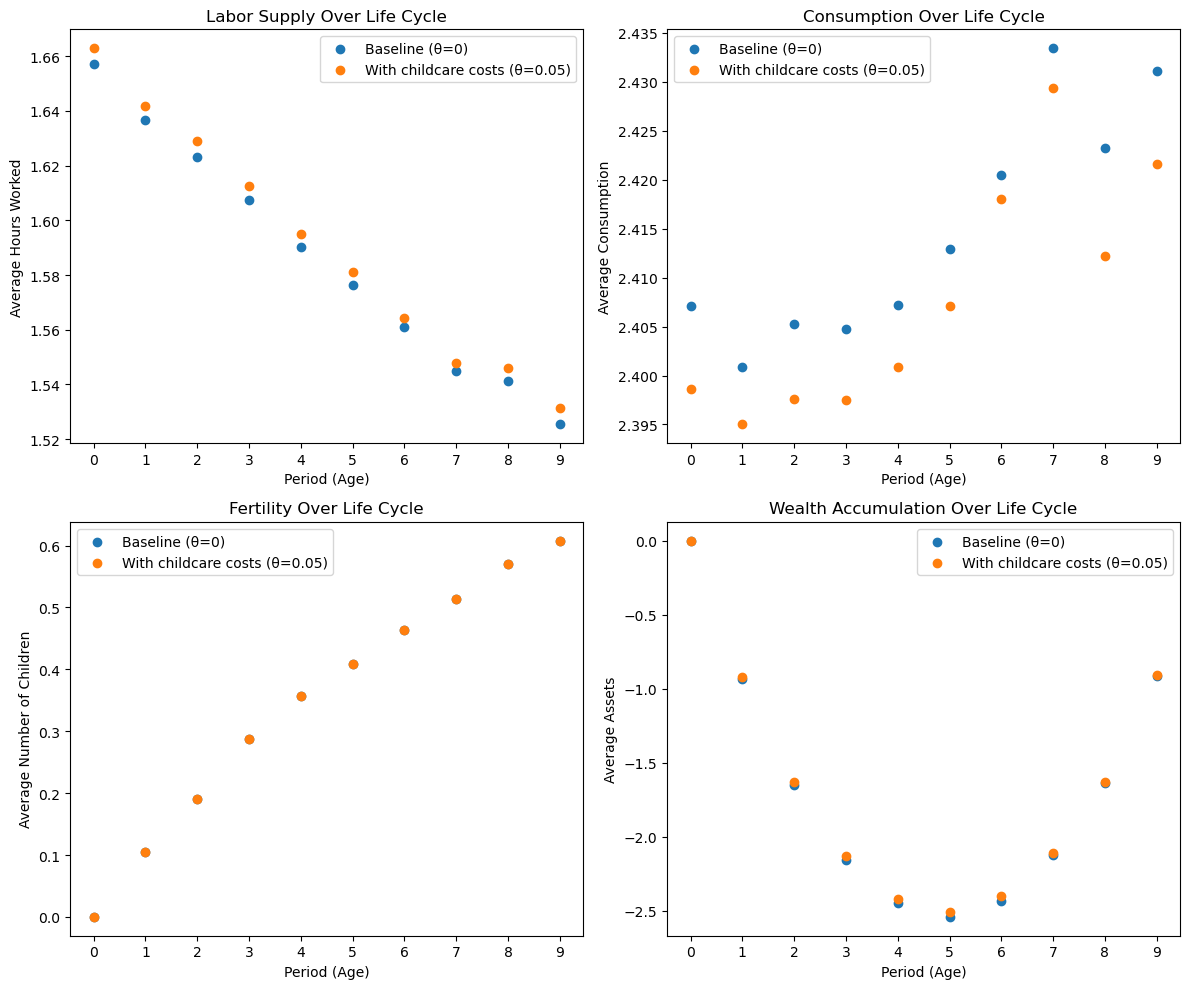
\includegraphics[width=0.5\linewidth]{Billeder/Lifecycle profiles_Q3_Ass1.png}
    \caption{Values when a child penalty is introduced.}
    \label{fig:placeholder}
\end{figure}
